\documentclass{scrreprt}
\usepackage{listings}
\usepackage{underscore}
\usepackage[bookmarks=true]{hyperref}
\usepackage[utf8]{inputenc}
\usepackage[english]{babel}
\usepackage{graphicx}
\usepackage{xcolor}
\usepackage{float}
\hypersetup{
    bookmarks=false,    % show bookmarks bar?
    pdftitle={Team 2 Policies},    % title
    pdfauthor={CMPT371 Team 2},                     % author
    pdfsubject={Policy},                        % subject of the document
    pdfkeywords={TeX, LaTeX, graphics, images, policy}, % list of keywords
    colorlinks=true,       % false: boxed links; true: colored links
    linkcolor=blue,       % color of internal links
    citecolor=black,       % color of links to bibliography
    filecolor=black,        % color of file links
    urlcolor=purple,        % color of external links
    linktoc=page            % only page is linked
}%
\def\myversion{1.0 }
\date{}
%\title
\usepackage{hyperref}
\begin{document}

\graphicspath{ {images/} }

\begin{flushright}
    \rule{16cm}{5pt}\vskip1cm
    \begin{bfseries}
        \Huge{TEAM 2 POLICY}\\
        \vspace{1.9cm}
        for\\
        \vspace{1.9cm}
        CMPT371\\
        \vspace{1.9cm}
        \LARGE{Version \myversion approved}\\
        \vspace{1.9cm}
        Prepared by Team 2\\
        \vspace{1.9cm}
        University of Saskatchewan\\
        \vspace{1.9cm}
        \today\\
    \end{bfseries}
\end{flushright}

\tableofcontents

\chapter{Policy}

\section{Members}

\begin{table}[h!]
\centering
\begin{tabular}{ |p{2cm}||p{8cm}|  }
    \hline
    \multicolumn{2}{|c|}{Team Roles} \\
    \hline
    Member & Roles\\
    \hline
    Evan & Project Lead\\
    Mesa & Design Lead\\
    Eileen & Test Lead\\
    Braunson & Build Master\\
    Kevin & Risk Officer, Development Team, Test Team\\
    Clinton & Test Team\\
    Anurag & Development Team, Test Team\\
    Amanda & Development Team\\
    Camille & Development Team\\
    \hline
\end{tabular}
\end{table}

\section{Roles and Responsibilities}

\subsection{Project Lead}

The project lead will be responsible for organizing meetings,
meeting with stakeholders, establishing priority of implementations, coordinating
between accountable positions, and other administrative work. 
Generally, the project lead will not directly code.
In cases of disagreements the project lead has executive decision making power.

\subsection{Design Lead}

The design lead is in charge of development. Their goal is
to complete the priorities set out by the stakeholder, organize
the development team to ensure cohesion, and selecting technologies
for use in the project. They should also ensure code quality and
work closely with the test lead and build master.

\subsection{Test Lead}

The test lead has to ensure there is sufficient test coverage
that adequately tests use cases of the stakeholder. They will
have oversight over the whole test team and is in charge of 
test plans.

\subsection{Build Master}

The build master ensures the build pipeline is maintained with
a server to deploy as staging and production environments. The
pipeline managed by the build master should include automating
tests, notifying group members of build issues, and ensuring
quality code is checked into the project.

\subsection{Risk Officer}

The risk officer is a rotating, part-time role which evaluates
risk continuously during project development. They are responsible
for documenting mitigation strategies and proactively taking
steps to reduce risks to the project. 

\section{Meetings}

Meetings and class room attendance is considered mandatory. 
If an individual cannot attend a meeting they are to notify the project lead ahead of time and must read the meeting minutes afterwards/when they are able to/at their earliest opportunity. If more than three meetings are missed in the course of the term that person must talk to Amanda, if any more meetings are missed, the team will talk to Dr. Osgood.

The first ten minutes of class will be used as an informal stand up.
If a team 2 member cannot attend they are to post on slack what they have done since last time and what they plan to do for next time. 

\section{Git}

The project follows the Git Flow paradigms. The only
modification is we do not strictly use release branches, releases
are tagged in master when a milestone is reached. 

For more information on how Git Flow works, see \href{https://www.atlassian.com/git/tutorials/comparing-workflows/gitflow-workflow}{here}.

All features must be reviewed via a pull request by at least two
people and the build must pass before it can be merged to the staging
environment. Every pull request should be associated with an issue that
has already been triaged.

\begin{figure}[H]
    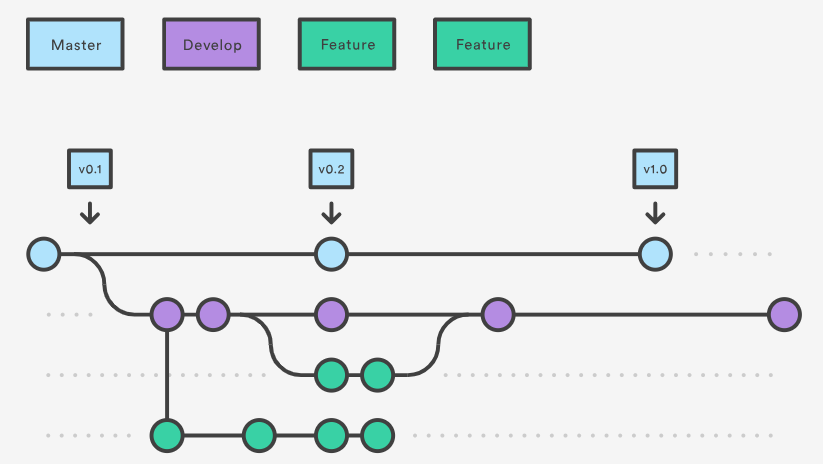
\includegraphics[width=\linewidth]{gitflow}
    \caption{A diagram of Git Flow.}
    \label{fig:gitflow}
\end{figure}

\section{Builds}

No member should knowingly push broken code to the repository.
All members should locally test the quality of their code before
pushing to the repository. 

\begin{figure}[H]
    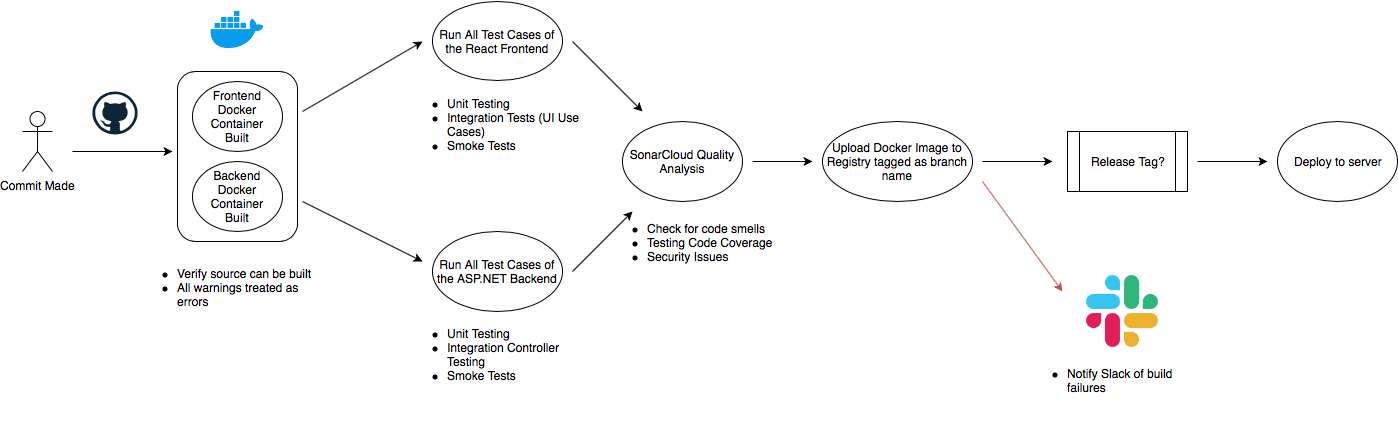
\includegraphics[width=\linewidth]{build-pipeline}
    \caption{A diagram of the build pipeline.}
    \label{fig:build}
\end{figure}

Some of the steps are subject to change as the project evolves.
Users who break the build are responsible for resolving the issue
before it is merged into the staging environment.

\section{Prototypes}

Prototypes should be placed in the prototypes directory with a README
file that details the objective of the prototype and the outcome. The
outcome will serve as a "lessons learned" for use in the project.

\end{document}